\chapter{Background}
This chapter lays down all the previous research which the project builds on. Before
going over the design decisions on the project we first need to understand this
background information and look at related work to see different approaches used
to solve the problem.

\section{Distributed Systems}
%% TODO: Find nice intro

A distributed system is a model in which processes running on running different
computers, which are connected together in a network, exchange messages to coordinate
their action, often resulting in the user thinking of the entire system as one single
unified computer.

A computer in the distibuted system is also alternatively referred to as a
processor or a node in the system. Each node in a distributed systems has its
own memory.

%% TODO: Structured in terms of client and servers

We will now go over a few concepts of distributed systems which will help us understand
the characteristics of the protocols that run on these systems. This will lay down the
groundwork for us to understand the Paxos protocol on which this project is based.

\subsection{Asynchronous Environment}
An asynchronous distributed system is one where there are no guarantees about the
timing and order in which events occur.

The clocks of each of the process in the system can be out of sync and may not be
accurate. Therefore, there can be no guarantees about the order in which events occur.

Further, messages sent by one process to another can be delayed for an arbitary period of time.

A protocol running in an asynchronous enviroment has to account for these conditions
in its design and try to achieve its goal without the guarantees of timed events.
An asynchronous environment is very common for a real world distributed system but
it also makes reasoning about the system harder because of the aforementioned properties.

\subsection{Fault Tolerance}
A fault tolerant distributed system is one which can continue to function correctly
despite the failure of some of its components. A 'failure' of a node or 'fault' in a node
means any unexpected behaviour from that node eg. not responding to messages, sending
corrupted messages.

Fault tolerance is one of the main reasons for using a distributed system as it
increases the chances of your application continuing to functioning correctly and
makes it more dependable. As Netflix mention on their blog
'Fault Tolerance is a Requirement, Not a Feature'.
%% TODO: Reference https://medium.com/netflix-techblog/fault-tolerance-in-a-high-volume-distributed-system-91ab4faae74a
With their Netflix API receiving more than 1 billion requests a day, they expect
that it is guaranteed that some of the components of their distributed system will fail.
Using a fault tolerant distributed system they are able to ensure that a small failure
in some components doesn't hinder the performance of the overall system, hence,
enabling them to achieve their uptime metrics.

Fault tolerant distributed system protocols are protocols which achieve their
goals despite the failure of some of the components of the distributed system they run on.
The protocol accounts for the failures and generally specifies the maximum number of
failures and the types of failures it can handle before it stops functioning correctly.

\subsection{State Machine Replication}
%% TODO: Reference https://www.cs.cornell.edu/fbs/publications/SMSurvey.pdf

For a client server model, the easiest way to implement it is to use one single server
which handles all the client request. Obviously this isn't the most robust solution
as if the single server fails, so does your service. To overcome the problem you
use a collection of servers each of which is a replica of the original single server and
ensure that each of these 'replicas' fails independantly, without effecting the other replicas.
This adds more fault tolerance.

State Machine Replication is method for creating a fault tolerant distributed system
by replicating servers and using protocols to coordinate the interactions of these
replicated servers with the client.

A State Machine $M$ can be defined as $M = \langle q_0, Q, I, O, \delta, \gamma \rangle$ where \\
$q_0$ is the starting state \\
$Q$ is the set of all possible states.
$I$ is set of all valid inputs
$O$ is the set of all valide outputs
$\delta$ is the state transition function, $\delta : I x Q -> Q$
$\gamma$ is the output function, $\gamma : I x Q -> O$

The state machine begins in the start state and transitions to other states and
produces outputs when it receives the inputs. The transition and output are found
using the transition and output functions. A deterministic state machine is one
whose state transition and output functions are injective, i.e. multiple
copies of the machine when given the same input, pass through the same order of states
and produce the same output in the same order.

The method of modelling a distributed system protocol as state transition system
is very common and is a critical component of this project as we will see soon when
we need to encode our protocol in Disel.

State machine replication involves modelling our single server, from the client
server model, and using multiple copies (replicas) of the same deterministic
state machine and providing all of them with the input from the client.
As long as one of the replicas does not crash, while resolving the request,
we can successfully return a response to the client.

%% TODO: Cover Byzantine Faults

\subsection{Consensus Protocols}
For handling faults in your distributed system you need to have replication.
This leads to the problem of making all these replicas agree with each other
to keep them consistent. Consensus protocols try to solve this problem.

Consensus protocols are the family of distibuted systems protocols which aim to
make a distributed network of processes agree on one result.

These protocols are of interest because of their numerous real world applications.
Let us take the example of a distributed database, which is a critical part of almost
all large scale real world applications. This distributed database will run
over a network of computers and everytime you use the database you aren't guaranteed
to be served by the same computer.

Suppose you add a file to the database. This action is performed by the processor that
was serving you 'add' request. Later when you want to retrieve the file from the database
you might be served by a different computer that did not perform the 'add' request. Inorder
for the new computer to know that the file exists in the database, you will need to use a
consensus protocol which helps all the computers in the network (which handle user
requests) agree upon the result that the file has been added to the database.

Popular consensus protocols include PageRank used by Google and the Blockchain
consensus protocol. George and Ilya verified a subset of the protocol in Coq in
their Toychain paper.
%% TODO: references


\section{Paxos}
Having understood the the main concepts behind distributed system protocols, we can
now finally get to the protocol at the heart of this project. Paxos is a family of
asynchronous, fault tolerant, consensus protocol which achieves consensus in a network
of unrealiable processes as long as a majority of them don't fail.

Paxos is used for state machine replication. Once you have multiple replicas
servicing client requests, how do you makes sure that all of these replicas agree
on what action to take? The solution is simply to use a consensus protocol like
Paxos to make all replicas agree on something.

Paxos has many variants but the one we will focus on is the one we actually prove
in Disel, single decree Paxos, also know as simple paxos. Simple Paxos is an algorithm
that helps a distributed network of processors to achieve consensus.
Consensus is achieved when the network of processor agree on a common value.

For simple paxos, we assume the following assumptions hold about the processors
and the environment, in order for the protocol to function correctly.
\begin{itemize}
  \item Processors communicate between each other by exchanging asynchronous messages between each other.
  \item Processors run at an arbitrary speed and may fail or restart. Handling this relates
    to the fault tolerant nature of paxos. Also, we assume that Byzantine faults don't occur.
    This means that all processors actually work together to try to achieve consensus on a value.
    There are variants of paxos which can also handle Byzantine failure buy not simple paxos.
    (This can be linked to the 'PBFT' paper which states that any algorithm handling
    Byzantine faults must have three phases. Simple paxos only has two phases.)
    %% TODO: References
\end{itemize}

As for fault tolerance of paxos, in order to handle a failure of upto $f$ processors,
we need to have a minimum $2f+1$ processors participating in the algorithm. This
means paxos functions correctly as long as a majority of the processors in the
network do not fail. We will see shortly why just a majority needs to function
correctly.

A processor participating in simple paxos, may have one or more of these three
different roles - proposer, acceptor or learner.
\begin{itemize}
  \item \textbf{Proposer} - A process acting as a proposer listens for client
    request and proposes a value which the network of processes tries to agree upon.
  \item \textbf{Acceptor} - acceptors receive proposed values from the proposers
    and then respond to them stating whether they are in a position to accept the value or not.
    For a proposed value to be accepted, a majority of all the existing acceptors
    have to accept the proposed value.
  \item \textbf{Learner} - The learner has to be informed when an acceptor accepts a value.
    The learner can then figure out when consensus has been achieved by calculating
    when a majority of acceptors have accepted the same proposal.
    Once the acceptors agree on a value, the learner may act on the value
    eg. Send request to client informing them about the agreed value.
\end{itemize}

% Safety Invariants:
% \begin{itemize}
%   \item A value can only be chosen after it has been proposed.
%   \item Only one value may be chosen.
% \end{itemize}

\vspace{-4mm}
\subsection{Choosing a Value}
For passing around the value to be chosen from one processor to the other,
a processor must send a 'proposal' to the other processor.
You can think of a proposal as just a tuple $\langle n, v \rangle$.
$n$ is just a natural number associated with a proposal which makes
it easy to keep track of all the different proposals.

A $quorum$ of acceptors is a subset of the set of all acceptors with length greater
than $N/2$ where $N$ is the length of the set of acceptors. A $quorum$ is just
a set denoting a majority of all the available acceptors.

\begin{quote}
Consensus is achieved when a proposal is accepted by a majority of acceptors.
\end{quote}

% There are a few requirements which are imposed for the algorithm to function correctly.
% The implementations of the algorithm ensure that these requirements are maintained.
% \begin{enumerate}
%   \item \textbf{R1} An acceptor must accept the first proposal it receives.
%   \item \textbf{R2} Once consensus has been achieved on a proposal,
%     $\langle n_1, v_1 \rangle$ then every other proposal, $\langle n_2, v_2 \rangle$,
%     on which consensus is achieved and has $n_2 > n_1$ will also have
%     $v_2 = v_1$.
% \end{enumerate}

% \textbf{R1} ensures that a value is agreed in the case when only a single value
% has been proposed by a single proposer. The most basic case is when you only have
% one acceptor. The acceptor can choose the first proposal that it receives from
% any of the proposers and then it can ignore the rest. The problem with using
% this is that if the single acceptor crashes then the algorithm won't make progress.
%
% So you need to have multiple acceptors but this is where the second problem arises.
% As multiple proposers might propose different values to different acceptors who
% might end up accepting different values.\textbf{R2} ensures that even though the
% acceptors might accept a proposal from a different proposer, all of the
% proposals accepted will have the same value. (Not sure about this)

\subsubsection{The Algorithm}
Simple paxos runs in rounds until consensus is achieved (a successful round
has occurred, where a majority of acceptors have accepted a proposal).
A successful round of the algorithm has two phases, each of which can
be subdivided into parts a, b.
%% TODO: Reference to proof of completion

\begin{itemize}
  \item \textbf{Phase 1a: Prepare Request.}
    A proposer sends a proposal
    $\langle n, v \rangle$ to each acceptor in any randomly chosen $quorum$ of acceptors.
    This first message that the proposer sends out is called a $prepare request$.
    As it the proposer tries to 'prepare' the acceptors to 'accept' a value in the future.
  \item \textbf{Phase 1b: Promise Response.}
    An acceptor on receiving a prepare request, responds with a $promise response$,
    if and only if the acceptor has not already sent a promise response with
    a proposal containing a proposal number $n'$ where $n' > n$.

    A promise response for proposal $\langle n, v \rangle$ is basically a
    guarantee (a 'promise') that this acceptor will not respond to any
    messages with proposals that have a proposal number $n'$ where $n' < n$.

    Thus, if an incoming prepare request has proposal number less than what the
    acceptor has already promised earlier, then the acceptor can ignore this
    prepare request by not responding to it. Although, for speeding up the
    protocol, the acceptor can send out a $nack response$ which tells the
    proposer to stop trying to achieve consensus with this proposal.

    If the acceptor has not sent any promise response before, then the body of
    the promise response can be empty, otherwise the acceptor must include the
    last proposal that it promised (before the current one) in the body of the
    message.
  \item \textbf{Phase 2b: Accept Request.}
    If the proposer successfully receives promise responses from a majority of
    acceptors, then it can send out an $accept request$. A accept request is
    a message containing a proposal which tells an acceptor to accept this
    proposal if it can.

    The proposer creates a new proposal, $\langle n, v' \rangle$ where $n$ is
    the same as in the proposal which the proposer sent in its prepare request.
    But, $v'$ is the value from the highest numbered proposal, selected from all
    the proposals that the proposer receives in the promise responses.
    If none of the promise responses received by the proposer contain a proposal,
    the proposer is free to set $v'$ to any value it likes.
    The proposer then sends this accept request with proposal $\langle n, v' \rangle$
    to another quorum of acceptors.
  \item \textbf{Phase 2b: Accepted Response.}
    Any acceptor that receives the accept request with proposal $\langle n, v \rangle$
    responds with an accepted response if and only if it hasn't already promised
    not to respond to any proposals with proposal number $n'$ where $n' > n$.
\end{itemize}

%% Not sure if algorithm implementation is required
%% can link to simulator in the appendix

\vspace{-4mm}
\subsection{Informing learner}
When consensus is achieved, a learner must be informed that a majority of acceptors
have agreed on a value. There are various ways to do this.

\begin{enumerate}
  \item Whenever an acceptor accepts a value, it should send the accepted proposal
    to all the learners. The learner will then know when a majority of acceptors
    have accepted the same value.
  \item We can have a distinguished learner which informs other learners about
    the choose value. The acceptors only need to inform this particular learner
    when they accept a value. This reduces number of messages sent but the
    distinguished learner becomes the single point of failure and also requires
    an additional round of sending messages where the distinguished learner informs
    other learners that a value has been chosen.
  \item We can use a set of distinguished learners. The acceptors inform these
    distinguished learners who then inform the other learners. This increases
    reliability but also increases the number of messages exchanged.
\end{enumerate}


\subsection{Inductive Invariant}
%% TODO: or more intuition, check Chapter 5 of http://adam.chlipala.net/frap/frap_book.pdf
A invariant in a program is a property of a program that always holds true,
from the start through to the end of execution of the program. An invariant can be for something
more specific like a function or even a loop. The only requirement is the property
described by the invariant should always hold before, during and after execution
of the part of that code.

The problem with using just an invariant like $x > 2$ is that, you may assume
that the invariant holds before the execution of the program, but you still
do not have a guarantee that this invariant will hold during and after the
execution of the program, i.e. in any state of the program.

Therefore, we need to make our invariants $inductive$. An inductive invariant
of a program, is an invariant which if it holds in a particular state $s$ of the
program, it is guaranteed to hold in all states of the program reachable from $s$.
Thus, having an inductive invariant that holds in the start state of a program
is much more useful, as we can be sure that the invariant will continue to
hold throughout and after the execution of the program.

This means that once you establish an inductive invariant from the given invariants
of a protocol and a starting state for the protocol in which the invariant holds,
in order to show that the protocol maintains the invariant, you only need to
prove the inductive invariant maintains the induction property over any possible state
transition in the protocol. This is exactly how you use an inductive invariant in
Disel.


\section{Disel}
%% TODO; Improve intro
Disel is a verification framework, built on top of the Coq theorem prover,
that enables one to prove the safety properties of a distributed protocol by
breaking down the protocol into its state space invariants and its atomic properties.

\subsection{Protocol Encoding}
We will now look at how Disel requires the state space of a protocol to be encoded in it.

%% TODO: copy image from Disel paper
%% TODO: cite Disel paper
"Each global system state $s$ is a finite partial mapping from protocol labels
$l \in \mathrm{\texttt{Lab}}$ to statelets. Each statelet represents a
protocol-specific component, consisting of a “message soup” MS and a per-node
local state (\texttt{DistLocState})."

%% TODO explain what a state is

As you can see from the image, a protocol $P$ in Disel is defined as a tuple
of the Coherence, the set of send transitions and the set of recieve transitions.
Let us now look at each of these components in detail.

A \texttt{Coherence} is a function that takes in a statelet and returns a proposition
indicating whether the statelet is valid or not. Thus, the coherence allows us
to impose constraints on the local state of each node and on the message soup.

A transition is defined as a tuple of consisting of the following:
\begin{enumerate}
  \item Tag - a unique natural number identifier for the message to be sent in the transition.
  \item Precondition - The constraints that are imposed on identity of the sender of the message,
    identity of the reciever is, the message that is being sent and on the local state of
    the sender/receiver (depending on whether it is a send transition/receive transition).
  \item Step function - Describes how the local state of the sender/reciever changes after
    making the transition.
\end{enumerate}

You can see in the code example below how the step function and pre condition
are encoded for sending the prepare request in Paxos.

\begin{lstlisting}
(* Changes in the Node state triggered upon send *)
Definition step_send (s: StateT) (to : nid) (p: proposal): StateT :=
    let: (e, rs) := s in
    match rs with
    ...
    (* Step function for the sending prepare request *)
    | PInit p' =>
      if acceptors == [:: to] (* if only one acceptor *)
      then (e, PWaitPrepResp [::] p')
      else (e, PSentPrep [:: to] p')
    ...
    | _ => (e, rs)
    end.

(* Precondition for send prepare request transition *)
Definition send_prepare_req_prec (p: StateT) (m: payload) :=
  (exists n psal, p = (n, PInit psal)) \/
  (exists n tos psal, p = (n, PSentPrep tos psal)).
\end{lstlisting}

\subsection{Protocol to Programs}
The state transitions that we implement in the protocol encoding phase, are the
first step towards creating executable programs using Disel.
We can then use the library of \textit{transition wrappers} provided by Disel
that allow one to decorate low level send/receive primitives with the transitions
that we have defined. These decorated primitives can later on be used to extract
code for executable programs. In Chapter 5, we will dive into the details of
how we extracted the code for our client application running Paxos.

The \texttt{send\_action\_wrapper} wrapper provided by Disel takes a send transition encoded
by us and returns a program that will send a message.
\begin{lstlisting}
Program Definition send_prepare_req psal to :=
  act (@send_action_wrapper W paxos p l (prEq paxos)
       (send_prepare_req_trans proposers acceptors) _ psal to).
\end{lstlisting}

The \texttt{tryrecv\_action\_wrapper} is similar but the main difference is that in
a received transition, we may received messages from any of the multiple protocols
that might be executing at the time. To address this problem, we need to check the
tag $t$ returned by the receive wrapper and ensure that this tag belongs to the
protocol that was specified in the wrapper. In the code example below, we check
that the received message is either a \texttt{promise\_resp} or a \texttt{nack\_resp}
both of which belong to the \texttt{paxos} protocol and are valid reponses to a
\texttt{prepare\_req}.
If an incoming message matches the conditions specified, the wrapper returns
\texttt{Some(from, m)} where $m$ is the message and $from$ is the sender. Otherwise
it returns \texttt{None}.

\begin{lstlisting}
(* Non blocking receive *)
Program Definition tryrecv_prepare_resp := act (@tryrecv_action_wrapper W p
      (* filter *)
      (fun k _ t b => (k == l) && ((t == promise_resp) || (t == nack_resp))) _).
\end{lstlisting}

These low level primitives can then be combined together for specifying the roles
of each node in the protocol. We can use the \texttt{send\_prepare\_req} to
come up with \texttt{send\_prepare\_req\_loop} which every proposer performs when
it starts up. These functions can then futher be combined together to give the
entire implementation of a node. \texttt{proposer\_round} below is the program
that each node acting a proposer executes.
\begin{lstlisting}
Program Definition send_prepare_req_loop e (psal: proposal):
  {(pinit: proposal)}, DHT [p, W]
  (fun i => loc i = st :-> (e, PInit pinit),
   fun r m => r = tt /\
              loc m = st :-> (e, PWaitPrepResp [::] pinit)) :=
  Do (ffix (fun (rec : send_prepare_req_loop_spec e) to_send =>
              Do (match to_send with
                  | to :: tos => send_prepare_req psal to ;; rec tos
                  | [::] => ret _ _ tt
                  end)) acceptors).

Program Definition proposer_round (psal: proposal):
  {(e : nat)}, DHT [p, W]
  (fun i => loc i = st :-> (e, PInit psal),
   fun res m => loc m = st :-> (e.+1, PAbort))
  :=
  Do (e <-- read_round;
      send_prepare_req_loop e psal;;
      recv_promises <-- receive_prepare_resp_loop e;
      check <-- check_promises recv_promises;
      if check
      then send_accept_reqs e (choose_highest_numbered_proposal psal recv_promises)
      else send_accept_reqs e [:: 0; 0]).
     (* If check fails then send an acc_req for (0, 0) which will never be
        accepted by any acceptor *)
\end{lstlisting}

Once this implementation has been finished in Disel we can use Disel's extraction
capabilities to extract the OCaml code for executing the program. (Outlined in Chapter 5)


\subsection{Approach to Mechanising Proofs in Disel}
\begin{figure}
\centering
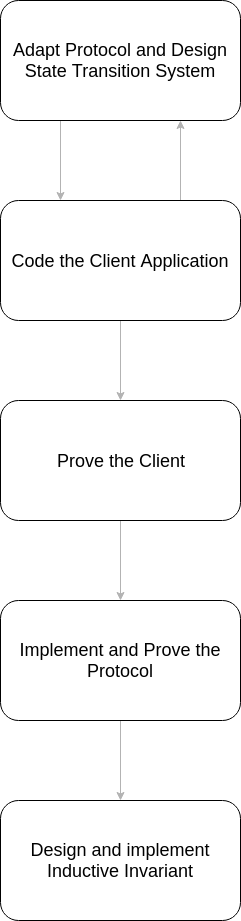
\includegraphics[width=0.2\textwidth]{figures/disel_workflow.png}
\caption{Disel Workflow
\label{fig:myInlineFigure}}
\end{figure}

% (1) Write code before proofs and run/test it;
%         (2) Prove that the code follows the protocol;
%         -----
%         (3) Write the protocol and prove invariants;
%
%
% You might want to have a diagram for this…
%
% Take a look at this paper (without going into details):
%
% https://www2.eecs.berkeley.edu/Pubs/TechRpts/2017/EECS-2017-163.pdf
%
% You might want to make a point that even without verifying inductive invariants, we already can get relatively strong correctness properties just by verifying (1)-(2).
%
% (1)-(2) is also sort of delivered by this work: https://eb.host.cs.st-andrews.ac.uk/writings/tdd-conc.pdf
%
% 1. I suggest you first
%   give a textual description with a lot of intuition about what kind of client
%   we are interested in and what properties it can observe that are guaranteed by the consensus.
% 2. Then you specify this property formally and sketch its proof.
%
% The client application does only need to have a couple of RPC-like procedures.
% It doesn't have to know about the entire protocol.
%
% Adapt Protocol and Design State transition system (iterate)
% | |
% Design and implement the Client Application (iterate)
% |
% Prove Client
% |
% Implement and prove Protocol
% |
% Design and implement Inductive Invariant

\subsubsection{1. Adapt Protocol and Design State transition system}
By adapting the protocol we try to focus on the 'core' parts of the protocol
and to do away with the 'conveniece' parts. For Paxos, this was focusing on the
part of the protocol that deals with achieving consensus and not looking at the
part where the learner is informed of the decision.

We also need to design state transition systems for the nodes that participate
in the protocol. This makes it easier for us to encode the protocol in Disel as
we already know which send and receive transitions we will need from each state
and thus can easily code the transition wrappers.

In chapter 4, we look go into the details of how we tackled this stage on our way
to mechanising the proof of Paxos.

\subsubsection{2. Code the client application}
Secondly, we need to think of a client application that uses the implemented protocol.
We need to design and implement a client that will demonstrate the properties of the
protocol that we want to prove. In case of Paxos, we designed a client
where nodes try to acheive consensus on one of the proposals that the proposer
is initialised with. This enabled us to see in action the stages of the protocol
that lead to consensus being achieved.

While using Disel, we often had to cycle between stage 1 and stage 2.
This is because while implementing the client, you realise things like, you are
missing one state for a node that is required in order for the protocol to progress.
While writing the client for Paxos, we realised that we were missing the \texttt{PAbort}
state for the proposer, which was necessary to signify when a proposer stops
participating in the protocol.

The process of cycling between stages 1 and 2 allow us to solidify our adapted
protocol. Doing this at an early stage (before starting the proofs)
also has the advantage of us not having to rewrite a lot of code that will also
break all the proofs relating to the change.

Additionally, implementing the client also helps us identify unnecessary stages
and transitions in the adapted protocol which were not needed to implement the
client. Reducing the number of states and transitions vastly reduces the amount
of things you will need to prove in the later stages.

\subsubsection{3. Prove the client}
The next stage involves proving that the code for the client actually follows
the adapted protocol. Thus, finishing the proofs in this stage gives us
confidence that our adapted protocol can actually be used to fullfill the role
which our client performs. In case of Paxos, this helped us realise that our
adapted protocol can be used to achieve consensus among the acceptors.

From this stage onwards, as we move to stages 4 and 5 we end up strengthening
the proof of our protocol. Finishing stage 4 completes the proof of the protocol
while reaching stage 5 actually adds an inductive invariant that stregthens the
proof of the protocol even further.

\subsubsection{4. Implement and prove the adapted protocol}
Having proved that our client follows the protocol, the next stage is for us
to actually finish the implementation of our protocol and to prove it. Finishing
stage 3, helped us be sure that the state transitions we have are enough for
realising the 'core' part of the protocol and that action of the client is proved.
Now we need to prove the protocol itself.

Finishing this stage meant that we have finished the proof of the protocol,
although we can only be sure that ...

\subsubsection{5. Design and implement Inductive Invariant}
In the proof of Paxos, we were only able to finish still stage 4. We designed
the inductive invariant but ran out of time to prove it.


\section{Related Work}
